\documentclass[aspectratio=169,11pt]{beamer}

\usetheme{Madrid}
\usecolortheme{default}
\setbeamertemplate{navigation symbols}{}
\setbeamertemplate{footline}[frame number]

\usepackage{amsmath,amssymb}
\usepackage{graphicx}
\usepackage{tikz}
\usetikzlibrary{positioning,calc}
\usetikzlibrary{arrows.meta,decorations.pathmorphing}

\definecolor{RamRed}{RGB}{190,40,45}
\definecolor{RamBlue}{RGB}{30,90,180}
\definecolor{SoftGray}{RGB}{245,245,245}
\definecolor{DarkGray}{RGB}{70,70,70}
\definecolor{MapGreen}{RGB}{48,150,95}
\definecolor{MapGold}{RGB}{235,180,45}

\setbeamercolor{title}{fg=DarkGray}
\setbeamercolor{frametitle}{fg=white,bg=RamBlue}
\setbeamercolor{structure}{fg=RamBlue}

\tikzset{
  v/.style={circle,draw=black,fill=white,inner sep=1.8pt},
  edge/.style={draw=RamBlue,line width=1.25pt},
  topic/.style={draw=black!30,fill=SoftGray,rounded corners=5pt,inner sep=7pt,
    text width=5.8cm,minimum height=1.65cm,align=left},
}


\usepackage{booktabs}
\tikzset{dot/.style={circle,fill=black,inner sep=2pt}, lab/.style={circle,draw=black,fill=white,inner sep=2pt,minimum size=6mm,font=\small},selected/.style={draw=RamRed,line width=2pt}}

\newcommand{\Def}[2]{\begin{block}{#1}#2\end{block}}
\newcommand{\Thm}[2]{\begin{block}{#1}#2\end{block}}
\renewcommand{\Proof}[1]{\begin{block}{Proof}\normalsize #1\end{block}}
\newcommand{\Question}[1]{\begin{block}{Question}#1\end{block}}
\renewcommand{\Example}[1]{\begin{block}{Example}#1\end{block}}
\newcommand{\fall}[2]{#1^{\underline{#2}}}
\newcommand{\rise}[2]{#1^{\overline{#2}}}
\newcommand{\stir}[2]{\left\{\begin{matrix}#1\\#2\end{matrix}\right\}}
\newcommand{\cyc}[2]{\left[\begin{matrix}#1\\#2\end{matrix}\right]}
\newcommand{\eul}[2]{\left\langle\begin{matrix}#1\\#2\end{matrix}\right\rangle}
\newcommand{\coef}[2]{[#1^{#2}]}
\newcommand{\gap}{\par\medskip}

\title{Recurrences and Catalan Numbers}
\author{Jeremy Quastel}\date{}\begin{document}
\begin{frame}[plain]\begin{center}{\Huge\bfseries Recurrences and Catalan Numbers}\par\vspace{.25cm}{\Large Section 2.6.4--2.6.6}\par\vspace{.15cm}{\large Harris--Hirst--Mossinghoff, \emph{Combinatorics and Graph Theory}}\par\vspace{.1cm}\resizebox{!}{2.7cm}{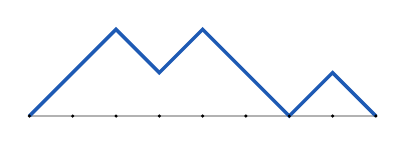
\begin{tikzpicture}[scale=.55]\draw[black!30](0,0)--(8,0);\draw[edge](0,0)--(1,1)--(2,2)--(3,1)--(4,2)--(5,1)--(6,0)--(7,1)--(8,0);\foreach \x in {0,...,8}{\fill(\x,0)circle(.04);}\end{tikzpicture}}\par\vspace{.25cm}Jeremy Quastel\end{center}\end{frame}
\begin{frame}[plain]\large \begin{center}{\Huge\bfseries Today\textquotesingle s lecture}\par\vspace{.5cm}\end{center}\begin{columns}[c,onlytextwidth]\begin{column}{.48\textwidth}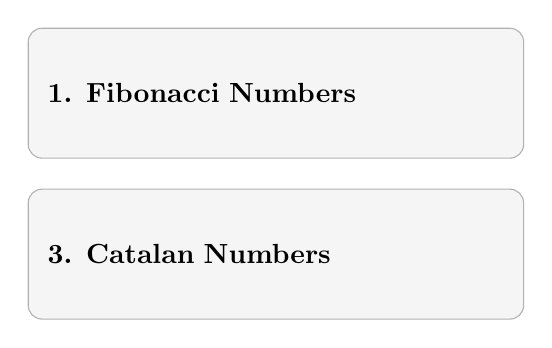
\begin{tikzpicture}\node[topic](a){\textbf{1. Fibonacci Numbers}};\node[topic,below=.38cm of a]{\textbf{3. Catalan Numbers}};\end{tikzpicture}\end{column}\begin{column}{.48\textwidth}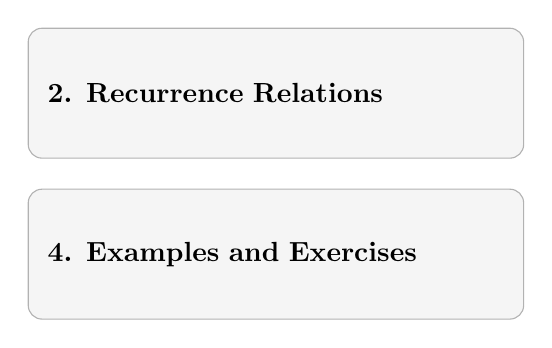
\begin{tikzpicture}\node[topic](a){\textbf{2. Recurrence Relations}};\node[topic,below=.38cm of a]{\textbf{4. Examples and Exercises}};\end{tikzpicture}\end{column}\end{columns}\end{frame}
\begin{frame}{Section 2.6.4: Fibonacci numbers}
\large
\Def{Fibonacci sequence}{Set $F_0=0$, $F_1=1$, and
\[F_n=F_{n-1}+F_{n-2}\qquad(n\geq2).\]}
\[0,1,1,2,3,5,8,13,21,34,\ldots\]
\gap A recurrence specifies each term using earlier terms, together with initial conditions.
\end{frame}
\begin{frame}{A tiling interpretation}
\large
\Question{How many ways can a board of length $n$ be tiled using tiles of lengths $1$ and $2$?}
\gap Let the answer be $t_n$. The final tile has length $1$ or $2$, leaving a board of length $n-1$ or $n-2$.
\[t_n=t_{n-1}+t_{n-2},\qquad t_0=t_1=1.\]
\end{frame}
\begin{frame}{Tilings and Fibonacci numbers}
\large
\Thm{Observation}{\[t_n=F_{n+1}.\]}
\Proof{The two sequences satisfy the same recurrence and have the same initial values after the index shift.}
\Example{For $n=4$, the tile-length words are $1111,112,121,211,22$. Thus $t_4=5=F_5$.}
\end{frame}
\begin{frame}{The Fibonacci generating function}
\large
Let
\[F(x)=\sum_{n\geq0}F_nx^n.\]
Multiply $F_n=F_{n-1}+F_{n-2}$ by $x^n$ and sum over $n\geq2$:
\[F(x)-x=xF(x)+x^2F(x).\]
\gap The subtracted term $x$ accounts for $F_1=1$.
\end{frame}
\begin{frame}{Solving for the generating function}
\large
\Thm{Formula}{\[F(x)=\frac{x}{1-x-x^2}.\]}
\gap For the tiling numbers,
\[T(x)=\sum_{n\geq0}t_nx^n=\frac1{1-x-x^2}.\]
\end{frame}
\begin{frame}{The characteristic roots}
\large
The equation $r^2=r+1$ has roots
\[\phi=\frac{1+\sqrt5}{2},\qquad\psi=\frac{1-\sqrt5}{2}.\]
\gap Since $\phi+\psi=1$ and $\phi\psi=-1$,
\[1-x-x^2=(1-\phi x)(1-\psi x).\]
\end{frame}
\begin{frame}{Partial fractions}
\large
\[\frac{x}{1-x-x^2}
=\frac1{\sqrt5}\left(\frac1{1-\phi x}-\frac1{1-\psi x}\right).\]
\gap Expand each denominator geometrically and compare coefficients.
\end{frame}
\begin{frame}{Binet's formula}
\large
\Thm{Theorem}{For $n\geq0$,
\[F_n=\frac{\phi^n-\psi^n}{\sqrt5}.\]}
\gap Although the expression contains irrational numbers, it is an integer because it equals the recursively defined Fibonacci number.
\end{frame}
\begin{frame}{Growth of the Fibonacci numbers}
\large
Since $|\psi|<1<\phi$,
\[F_n\sim\frac{\phi^n}{\sqrt5}.\]
\gap In particular,
\[\lim_{n\to\infty}\frac{F_{n+1}}{F_n}=\phi.\]
\gap The larger characteristic root determines the leading growth.
\end{frame}
\begin{frame}{A Fibonacci sum}
\large
\Thm{Identity}{For $n\geq0$,
\[\sum_{j=0}^nF_j=F_{n+2}-1.\]}
\Proof{Rewrite the recurrence as $F_j=F_{j+2}-F_{j+1}$ and sum. The right-hand side telescopes to $F_{n+2}-F_1$.}
\end{frame}
\begin{frame}{A sum of squares}
\large
\Thm{Identity}{\[\sum_{j=0}^nF_j^2=F_nF_{n+1}.\]}
\Proof{The statement holds at $n=0$. If it holds at $n-1$, add $F_n^2$:
\[F_{n-1}F_n+F_n^2=F_n(F_{n-1}+F_n)=F_nF_{n+1}.\]}
\end{frame}
\begin{frame}{Section 2.6.5: Recurrence relations}
\large
\Def{Linear homogeneous recurrence}{A recurrence of order $d$ with constant coefficients has the form
\[a_n=c_1a_{n-1}+\cdots+c_da_{n-d}.\]}
\gap The first $d$ values determine the sequence. We begin with order $2$.
\end{frame}
\begin{frame}{The characteristic equation}
\large
For
\[a_n=ua_{n-1}+va_{n-2},\]
try a solution $a_n=r^n$. Substitution leads to
\[r^2-ur-v=0.\]
\gap When the roots $r_1,r_2$ are distinct, the general solution is
\[a_n=Ar_1^n+Br_2^n.\]
\end{frame}
\begin{frame}{Why two constants suffice}
\large
\Proof{Each root gives a solution, and linear combinations of solutions are solutions. Distinct roots let us solve uniquely for $A,B$ from $a_0,a_1$.\gap The resulting sequence agrees with the required sequence in its first two terms and satisfies the same recurrence. Induction makes the two sequences identical.}
\end{frame}
\begin{frame}{An example with distinct roots}
\large
\Question{Solve $a_n=5a_{n-1}-6a_{n-2}$ with $a_0=2$, $a_1=5$.}
\gap The characteristic polynomial factors as
\[r^2-5r+6=(r-2)(r-3).\]
So $a_n=A2^n+B3^n$.
\end{frame}
\begin{frame}{Determining the constants}
\large
\[A+B=2,\qquad2A+3B=5.\]
Hence $A=B=1$, and
\[a_n=2^n+3^n.\]
\gap Check: $a_2=13=5\cdot5-6\cdot2$.
\end{frame}
\begin{frame}{Repeated roots}
\large
\Thm{Order-two repeated-root case}{If the characteristic polynomial is $(r-\lambda)^2$ with $\lambda\ne0$, then
\[a_n=(A+Bn)\lambda^n.\]}
\gap The extra factor $n$ supplies a second independent solution.
\gap For a root of multiplicity $m$, the corresponding terms involve $n^j\lambda^n$ for $0\leq j<m$.
\end{frame}
\begin{frame}{A repeated-root example}
\large
\Question{Solve $a_n=4a_{n-1}-4a_{n-2}$ with $a_0=1$, $a_1=4$.}
\gap The polynomial is $(r-2)^2$, so $a_n=(A+Bn)2^n$.
\gap Initial values give $A=1$ and $2(1+B)=4$. Therefore
\[a_n=(n+1)2^n.\]
\end{frame}
\begin{frame}{Generating functions for recurrences}
\large
\Thm{Order-two formula}{If $a_n=ua_{n-1}+va_{n-2}$ for $n\geq2$, then
\[A(x)=\frac{a_0+(a_1-ua_0)x}{1-ux-vx^2}.\]}
\Proof{Sum the recurrence after multiplying by $x^n$:
\[A-a_0-a_1x=ux(A-a_0)+vx^2A.\]
Rearrange.}
\end{frame}
\begin{frame}{The repeated-root example revisited}
\large
\[A(x)=\frac{1+(4-4)x}{1-4x+4x^2}=\frac1{(1-2x)^2}.\]
\gap Using $(1-z)^{-2}=\sum_{n\geq0}(n+1)z^n$ gives
\[a_n=(n+1)2^n.\]
\gap Partial fractions explain why repeated roots produce polynomial factors in $n$.
\end{frame}
\begin{frame}{Nonhomogeneous recurrences}
\large
\Def{Definition}{A recurrence is nonhomogeneous when an additional term depends on $n$:
\[a_n=c_1a_{n-1}+\cdots+c_da_{n-d}+b_n.\]}
\gap One method is to find a particular solution and add a general solution of the associated homogeneous recurrence.
\end{frame}
\begin{frame}{A constant forcing term}
\large
\Question{Solve $a_n=2a_{n-1}+1$, $a_0=0$.}
\gap Set $b_n=a_n+1$. Then $b_n=2b_{n-1}$ and $b_0=1$, giving
\[a_n=2^n-1.\]
\end{frame}
\begin{frame}{A resonant forcing term}
\large
\Question{Solve $a_n=2a_{n-1}+2^n$, $a_0=0$.}
\gap Divide by $2^n$ and set $b_n=a_n/2^n$:
\[b_n=b_{n-1}+1,\qquad b_0=0.\]
Thus $b_n=n$ and $a_n=n2^n$.
\end{frame}
\begin{frame}{Recurrences from counting}
\large
\Question{Let $a_n$ count binary words of length $n$ with no consecutive ones. Find a recurrence.}
\gap A word ends in $0$, or ends in $01$ if its length is at least $2$.
\[a_n=a_{n-1}+a_{n-2},\qquad a_0=1,\ a_1=2.\]
Thus $a_n=F_{n+2}$.
\end{frame}
\begin{frame}{Section 2.6.6: Catalan numbers}
\large
\Question{How many strings of $n$ opening and $n$ closing parentheses are correctly matched?}
\gap At every initial segment, the number of opening parentheses must be at least the number of closing parentheses.
\gap For $n=3$, there are five:
\[\texttt{((()))},\ \texttt{(()())},\ \texttt{(())()},\ \texttt{()(())},\ \texttt{()()()}.\]
\end{frame}
\begin{frame}{Dyck paths}
\large
\Def{Dyck path}{A Dyck path of semilength $n$ uses $n$ up steps $(1,1)$ and $n$ down steps $(1,-1)$ and never goes below height zero.}
\begin{center}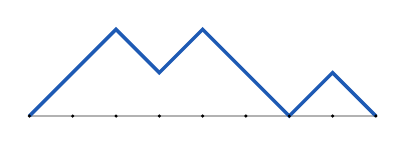
\begin{tikzpicture}[scale=.55]\draw[black!30](0,0)--(8,0);\draw[edge](0,0)--(1,1)--(2,2)--(3,1)--(4,2)--(5,1)--(6,0)--(7,1)--(8,0);\foreach \x in {0,...,8}{\fill(\x,0)circle(.04);}\end{tikzpicture}\end{center}
\begin{center}Opening parentheses are up steps; closing parentheses are down steps.\end{center}
\end{frame}
\begin{frame}{The Catalan sequence}
\large
Let $C_n$ count Dyck paths of semilength $n$, with $C_0=1$ for the empty path.
\[C_0,C_1,C_2,C_3,C_4,C_5=1,1,2,5,14,42.\]
\gap Decomposing a path at its first return to height zero gives a recurrence.
\end{frame}
\begin{frame}{The first-return decomposition}
\large
Every nonempty Dyck path has a unique form
\[U\,P\,D\,Q,\]
where the displayed $D$ is the first return to height zero, and $P,Q$ are Dyck paths after shifting $P$ down by one unit.
\gap If $P$ has semilength $i$, then $Q$ has semilength $n-1-i$.
\end{frame}
\begin{frame}{The Catalan recurrence}
\large
\Thm{Recurrence}{For $n\geq1$,
\[C_n=\sum_{i=0}^{n-1}C_iC_{n-1-i},\qquad C_0=1.\]}
\Example{$C_4=C_0C_3+C_1C_2+C_2C_1+C_3C_0=5+2+2+5=14$.}
\end{frame}
\begin{frame}{The Catalan generating function}
\large
Let $C(x)=\sum_{n\geq0}C_nx^n$. The recurrence becomes
\[C(x)-1=xC(x)^2.\]
Solving the quadratic and choosing the branch with constant term $1$ gives
\[C(x)=\frac{1-\sqrt{1-4x}}{2x}.\]
\end{frame}
\begin{frame}{A closed formula}
\large
\Thm{Catalan formula}{For $n\geq0$,
\[C_n=\frac1{n+1}\binom{2n}n.\]}
\gap We prove this directly by subtracting paths that fall below the axis from all paths with $n$ up and $n$ down steps.
\end{frame}
\begin{frame}{Reflecting a bad path}
\large
\Proof{There are $\binom{2n}n$ unrestricted paths from height $0$ to height $0$.\gap For a bad path, reflect its initial segment through the first step reaching height $-1$, interchanging up and down steps. That segment had one more down step than up step; after reflection the whole path has $n+1$ up and $n-1$ down steps.}
\end{frame}
\begin{frame}{The reflection bijection}
\large
\Proof{Conversely, a path with $n+1$ up and $n-1$ down steps ends at height $2$ and has a first visit to height $1$. Reflect its initial segment through that visit. This reverses the construction.\gap Therefore bad paths number $\binom{2n}{n-1}$, and
\[C_n=\binom{2n}n-\binom{2n}{n-1}=\frac1{n+1}\binom{2n}n.\]}
\end{frame}
\begin{frame}{Triangulations of a polygon}
\large
\Thm{Catalan interpretation}{A convex polygon with $n+2$ vertices has $C_n$ triangulations.}
\Proof{Fix one boundary edge. The triangle incident with it has a unique third vertex, splitting the remaining polygon into two smaller polygons. Summing over that vertex gives the Catalan recurrence, with the empty region counted as $1$.}
\end{frame}
\begin{frame}{Other Catalan families}
\large
\begin{itemize}
\item Correctly matched parentheses with $n$ pairs.
\item Dyck paths of semilength $n$.
\item Triangulations of a convex $(n+2)$-gon.
\item Noncrossing perfect matchings of $2n$ points on a circle.
\item Rooted ordered full binary trees with $n$ internal vertices.
\end{itemize}
\gap Each family admits the same decomposition into a pair of smaller objects.
\end{frame}
\begin{frame}{Practice}
\large
\Question{How many correctly matched parenthesis strings with four pairs have their first return to balance zero after the fourth symbol?}
\gap In $U P D Q$, determine the semilengths of $P$ and $Q$.
\end{frame}
\begin{frame}{Practice: solution}
\large
The initial block $UPD$ has two pairs, so $P$ has one pair. The remainder $Q$ has two pairs.
\[C_1C_2=1\cdot2=2.\]
\gap The strings are \texttt{(())(())} and \texttt{(())()()}.
\end{frame}
\begin{frame}{Summary}
\large
\begin{itemize}
\item Initial conditions and a recurrence determine a sequence.
\item Characteristic roots and generating functions solve constant-coefficient linear recurrences.
\item Repeated roots create polynomial factors.
\item Catalan objects split recursively into two smaller objects and satisfy a convolution recurrence.
\end{itemize}
\end{frame}
\begin{frame}{Next time: Permutation Groups and Burnside\textquotesingle s Lemma}\begin{center}{\Huge Permutation Groups and Burnside\textquotesingle s Lemma}\end{center}\end{frame}
\end{document}